%%%%%%%%%%%%%%%%%%%%%%%%%%%%%%%%%%%%%%%%%
%
% (c) 2020 by Jennifer Laaser
%
% This work is licensed under the Creative Commons Attribution-NonCommercial-ShareAlike 4.0 International License. To view a copy of this license, visit http://creativecommons.org/licenses/by-nc-sa/4.0/ or send a letter to Creative Commons, PO Box 1866, Mountain View, CA 94042, USA.
%
% The current source for these materials is accessible on Github: https://github.com/jlaaser/pogil-polymers
%
%%%%%%%%%%%%%%%%%%%%%%%%%%%%%%%%%%%%%%%%%

\documentclass[instructor,handout]{pogil}

%%%%%%%%%%%%%%%%% DOCUMENT INFORMATION %%%%%%%%%%%%%%%%%%%%%%%%

\copyrightshort{
\includegraphics[width=0.1\textwidth]{by-nc-sa} J. Laaser 2020}

%%%%%%%%%%%%%%%%%%%%%%%%%%%%%%%%%%%%%%%%%%%%%%%%%%%%%%%%%%%%%%%%%
%%%%%%%%%%%%%%%%%%%%%%%%%%%%%%%%%%%%%%%%%%%%%%%%%%%%%%%%%%%%%%%%%

\begin{document}
	
% to change the activity output in the pdf, change this to the file path for the activity you want to include:
%%%%%%%%%%%%%%%%%%%%%%%%%%%%%%%%%%%%%%%%%%
%
% (c) 2018 by Jennifer Laaser
%
% This work is licensed under the Creative Commons Attribution-NonCommercial-ShareAlike 4.0 International License. To view a copy of this license, visit http://creativecommons.org/licenses/by-nc-sa/4.0/ or send a letter to Creative Commons, PO Box 1866, Mountain View, CA 94042, USA.
%
% The current source for these materials is accessible on Github: https://github.com/jlaaser/pogil-polymers
%
%%%%%%%%%%%%%%%%%%%%%%%%%%%%%%%%%%%%%%%%%

\section{Activity Template}
\renewcommand{\figpath}{content/figs}

\textbf{Focus question:} Put a central question for the students to consider through this exercise here.

\subsection{Model 1:  ABC}

Here is the first model for students to consider

% to include images, put them in the folder specified by figpath and then use:
%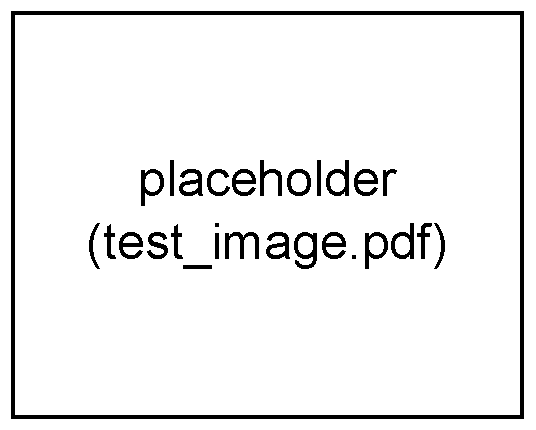
\includegraphics[width=0.8\textwidth]{\figpath/test_image.pdf}

\subsection{Critical Thinking Questions}

	\begin{enumerate}
		\item First question?
		\item Second question?
	\end{enumerate}

\subsection{Model 2: DEF}

\subsection{Critical Thinking Questions}

	\begin{enumerate}
		\item First question?
		\item Second question?
	\end{enumerate}

\subsection{Exercises}

	After class, \textbf{read} the following sections of your textbook:
	
	\begin{enumerate}
		\item First section
		\item Second section
	\end{enumerate}
	
	Then, do the following exercises:
	
	\begin{enumerate}
		\item First exercise
		\item Second exercise
	\end{enumerate}
%%%%%%%%%%%%%%%%%%%%%%%%%%%%%%%%%%%%%%%%%%
%
% (c) 2019 by Jennifer Laaser
%
% This work is licensed under the Creative Commons Attribution-NonCommercial-ShareAlike 4.0 International License. To view a copy of this license, visit http://creativecommons.org/licenses/by-nc-sa/4.0/ or send a letter to Creative Commons, PO Box 1866, Mountain View, CA 94042, USA.
%
% The current source for these materials is accessible on Github: https://github.com/jlaaser/pogil-polymers
%
%%%%%%%%%%%%%%%%%%%%%%%%%%%%%%%%%%%%%%%%%

\renewcommand{\figpath}{content/polymchem/networks/network-synth/figs}
\renewcommand{\labelbase}{network-synth}

\begin{activity}[Synthesis of Polymer Networks]

\begin{instructornotes}
	This activity introduces students to concepts related to the synthesis of polymer networks.
	
	After completing this activity, students will be able to:
	\begin{enumerate}
		\item \dots
	\end{enumerate}
	
	\subsection*{Activity summary:}
	\begin{itemize}
		\item \textbf{Activity type:} Learning Cycle
		\item \textbf{Content goals:} Synthesis of Polymer Networks
		\item \textbf{Process goals:} %https://pogil.org/uploads/attachments/cj54b5yts006cklx4hh758htf-process-skills-official-pogil-list-2015-original.pdf
			written communication, critical thinking, information processing
		\item \textbf{Duration:} TBD
		\item \textbf{Instructor preparation required:} none beyond knowledge of relevant content
		\item \textbf{Related textbook chapters:}
			\begin{itemize}
				\item \emph{Polymer Chemistry} (Hiemenz \& Lodge): section NNN
			\end{itemize}
		%\item \textbf{Facilitation notes:}
		%	\begin{itemize}
		%		\item \dots
		%	\end{itemize}
	\end{itemize}
	
\end{instructornotes}


\begin{model}[Linking Polymer Strands]
	\label{\labelbase:mdl:linking}

	One way to synthesize a polymer network is to crosslink pre-formed polymer chains.
	
	Consider the following collection of polymer chains:
	
	\centerline{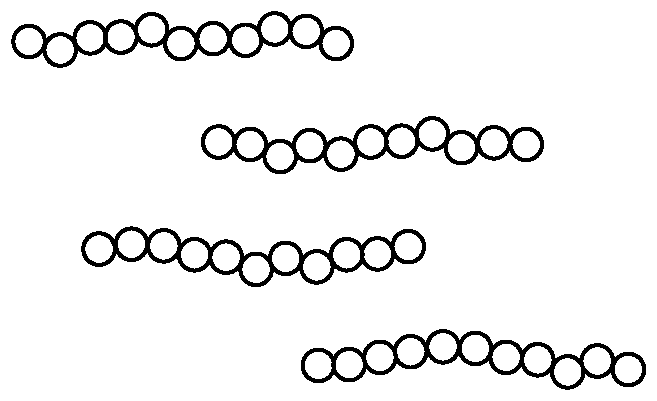
\includegraphics[width=0.5\textwidth]{\figpath/Model1_linking_blank.pdf}}
	
	To form a network, the chains must be crosslinked together to form a single large molecule:
	
	\centerline{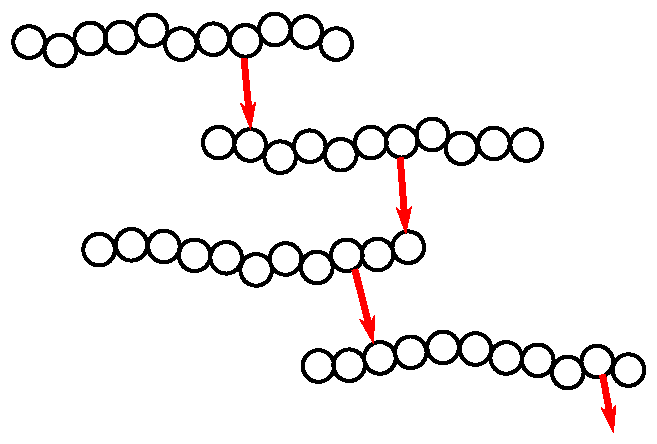
\includegraphics[width=0.5\textwidth]{\figpath/Model1_linking_arrows.pdf}}
	
	Here, we have drawn the crosslinks as arrows to make the analysis easier, but in practice, crosslinks do not have a specific orientation.
	
\end{model}


\begin{ctqs}

	\question In the picture shown in Model \ref{\labelbase:mdl:linking}, what is the \emph{minimum} number of ``outgoing'' crosslinks (arrows pointing away from the chain) that each polymer chain must have in order to allow a network to form?
	
		\begin{solution}[0.5in]
		
			one (each strand must link to the next to link all of the strands into a single molecule)
			
		\end{solution}
		
	\question If each polymer chain has $N$ monomers, what is the \emph{minimum fraction} of monomers, $x_c$, that must form an outgoing crosslink in order for a network to form?
	
		\begin{solution}[0.5in]
			$x_c = \frac{1}{N}$
		\end{solution}
		
	\question Briefly describe, in 2-3 complete sentences, how you could determine the minimum amount of crosslinker necessary to form a network from a polymer with molecular weight $M_n$.
	
		\begin{solution}[2in]
			First, take the molecular weight and divide by the monomer mass $M_0$ to find the degree of polymerization $N$.  Then, calculate the minimum fraction of monomers that need to be crosslinked to form a network using $x_c = \frac{1}{N_n}$.  Finally, use the total mass (or total number of moles) of monomer to calculate the total mass (or total number of moles) of crosslinker corresponding to this fraction.
		\end{solution}
		
	%\question Suppose a fraction $x > x_c$ of the monomers form outgoing crosslinks.
	
	%	\begin{enumerate}
	%		\item On average, how many monomers do you expect to find between outgoing crosslinks?
			
	%		\item On average, how many ``incoming'' crosslinks will that same set of monomers have?
	%		
	%		\item On average, 
	%	\end{enumerate}
	
\end{ctqs}

\begin{model}[Step-Growth Network Synthesis]

	A second way to synthesize a network is via step-growth polymerization of multi-functional monomers.
	
	For example, a step-growth polymerization of a difunctional ``AA'' monomer with a trifunctional ``B$_3$'' monomer might yield a network as follows:
	
	\centerline{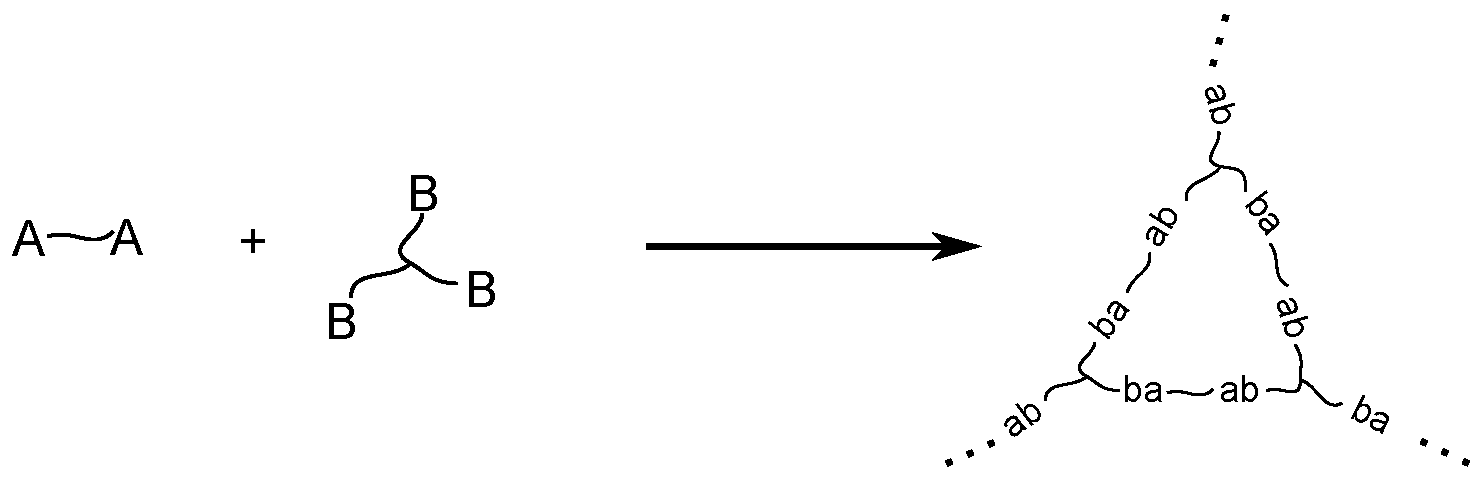
\includegraphics[width=0.7\textwidth]{\figpath/Model2_A2B3network.pdf}}

\end{model}

\begin{ctqs}

	\question Suppose that you started this reaction with 3 AA-type monomers and 2 $B_3$ monomers, as shown below:
	
	\vspace{6pt}
		\centerline{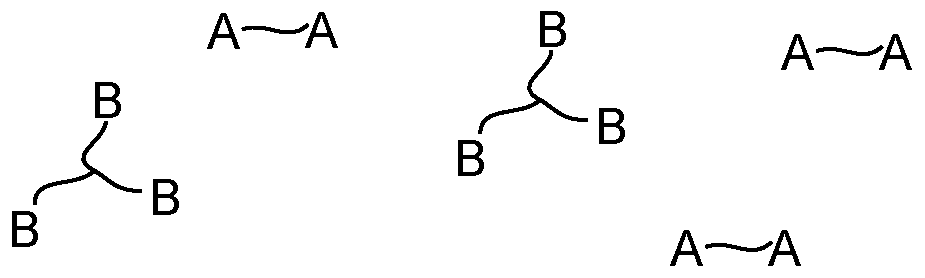
\includegraphics[width=0.5\textwidth]{\figpath/Model2_A2B3_initial.pdf}}
	
		\begin{enumerate}
			\item How many \emph{molecules} are present in the initial reaction mixture?
			
				\begin{solution}[0.75in]
					5
				\end{solution}
			
			\item How many \emph{reactive functional groups} are present in the initial reaction mixture?  For the purposes of this question, count both the A and B reactive groups.
			
				\begin{solution}[0.5in]
					12 (6 from AA-type monomers, 6 from B3-type monomers)
				\end{solution}
			
		\end{enumerate}
		
	\question Now, suppose we move two ``steps'' forward in the reaction (i.e. we form two ``ab'' bonds).
	
		\begin{enumerate}
		
			\item Draw one possible structure that could occur after two bond-forming reactions have taken place:
			
				\begin{solution}[1.75in]
				
					(student answers may vary)
					
				\end{solution}
			
			\item How many \emph{molecules} are present after two bond-forming reactions have taken place?
			
				\begin{solution}[0.5in]
					3
				\end{solution}
			
			\item How many functional groups \emph{have reacted} after two bond-forming reactions have taken place?  For the purposes of this question count both the a's and the b's.
			
				\begin{solution}[0.5in]
					4
				\end{solution}
				
			\item Calculate the extent of reaction, $p$ (fraction of functional groups that have reacted), and the number-average degree of polymerization, $N_n$, for this state of the reaction.
			
				\begin{solution}[2.25in]
					$p = \frac{\text{\# reacted}}{\text{initial \# of reactive groups}} = \frac{4}{12} = 0.33$
					
					$N_n = \frac{\text{initial \# of molecules}}{\text{final \# of molecules}} = \frac{5}{3} = 1.67$
					
					Note: students may get stuck on $N_n$.  Give them a hint if necessary.
				\end{solution}
		\end{enumerate}

	\question More generally, suppose that you initially have $n_0$ molecules that have an average of $\langle f\rangle$ reactive groups per monomer.  
	
		What is the \emph{total number} of reactive functional groups at the start of your reaction?
	
			\begin{solution}[1in]
				$n_0 \langle f \rangle$
			\end{solution}
			
	\question Suppose that at some time later, there are $n$ molecules in the reaction mixture.
	
		\begin{enumerate}
		
			\item How many bond-forming reactions must have occurred to reach this point?  \emph{(Hint: how much does the number of molecules in the reaction change each time a bond-forming reaction happens?)}
			
				\begin{solution}[0.65in]
					$n_0 - n$ (each bond-forming reaction reduces the number of molecules by one, so if we have dropped from $n_0$ to $n$ molecules, we must have undergone $n_0-n$ bond-forming reactions)
				\end{solution}
		
			\item How many functional groups must have reacted to reach this point?
			
				\begin{solution}[0.65in]
					$2(n_0-n)$ (each bond-forming reaction uses up two reactive groups)
				\end{solution}
			
			\question What is the number-average degree of polymerization at this point in the reaction?
			
				\begin{solution}[0.65in]
					$N_n = \frac{n_0}{n}$
				\end{solution}
			
			\question What is the extent of reaction at this point in the reaction?
			
				\begin{solution}[0.65in]
					$p = \frac{2(n_0-n)}{n_0\langle f \rangle}$
				\end{solution}
		
		\end{enumerate}
	
\end{ctqs}

\begin{infobox}
	Combining the expressions you derived for $p$ and $N_n$, above, it is possible to show that
	\begin{equation*}
		N_n = \frac{2}{2-p\langle f \rangle}
	\end{equation*}
	This relationship is referred to as the \emph{Carothers equation}.
\end{infobox}

\begin{ctqs}
	\question As the network begins to form, all of the monomers effectively link into a single large molecule.  What must happen to $N_n$ in this case?  Briefly explain your group's reasoning in 1-2 complete sentences.
	
		\begin{solution}[2in]
			As the monomers all link into a single molecule, $N_n$ must become very large.  In the limit of having a large number of initial monomers, $N_n$ effectively goes to infinity.
			
			\emph{Note: strictly speaking, it is actually $N_w$ that must approach infinity, but this distinction is a subtle point and not necessary for this activity.}
		\end{solution}
	
	\question What must be true about the value of $2-p\langle f \rangle$ in order for $N_n\to\infty$?
	
		\begin{solution}[1.5in]
			$2-p\langle f\rangle = 0$ (value of the fraction blows up if the denominator is zero)
		\end{solution}
	
	\question Rearrange your answer to the previous question to find the minimum extent of reaction at which a network will form.
	
		\begin{solution}[1in]
			$p = \frac{2}{\langle f \rangle}$
		\end{solution}
\end{ctqs}


\begin{exercises}

%	\exercise Exercise about stoichiometric imbalance in network synthesis?
	
	%\exercise In Model \ref{\labelbase:mdl:linking}, you considered formation of networks by linking together pre-formed polymer chains.  However, the same analysis can be used to understand networks formed by chain-growth polymerization of mixtures containing difunctional monomers.
	
	%	\begin{enumerate}
	%		\item 
	%	\end{enuemrate}	
	
	\exercise Consider the AA+BB-type step-growth polymerizations that you learned about earlier this term.
	
		\begin{enumerate}
			\item In an AA+BB-type polymerization, what is the average number of reactive functional groups per molecule?
			
			\item Show that, with this value of $\langle f\rangle$, the Carothers equation simplifies to the version you learned for step-growth polymerizations.
		\end{enumerate}	
	
\end{exercises}


%\begin{problems}
%
%	\problem First exercise
%	\problem Second exercise
%	
%\end{problems}


	
\end{activity}
%%%%%%%%%%%%%%%%%%%%%%%%%%%%%%%%%%%%%%%%%
%
% (c) 2019 by Jennifer Laaser
%
% This work is licensed under the Creative Commons Attribution-NonCommercial-ShareAlike 4.0 International License. To view a copy of this license, visit http://creativecommons.org/licenses/by-nc-sa/4.0/ or send a letter to Creative Commons, PO Box 1866, Mountain View, CA 94042, USA.
%
% The current source for these materials is accessible on Github: https://github.com/jlaaser/pogil-polymers
%
%%%%%%%%%%%%%%%%%%%%%%%%%%%%%%%%%%%%%%%%%

\renewcommand{\figpath}{content/polymphys/mechanical-properties/elasticity/figs}
\renewcommand{\labelbase}{elasticity}

\begin{activity}[Elasticity of Polymer Networks]

\begin{instructornotes}
	This activity introduces students to concepts related to the tensile properties of polymer networks.
	
	After completing this activity, students will be able to:
	\begin{enumerate}
		\item \dots
	\end{enumerate}
	
	\subsection*{Activity summary:}
	\begin{itemize}
		\item \textbf{Activity type:} Learning Cycle
		\item \textbf{Content goals:} Tensile Properties of Polymer Networks
		\item \textbf{Process goals:} %https://pogil.org/uploads/attachments/cj54b5yts006cklx4hh758htf-process-skills-official-pogil-list-2015-original.pdf
			written communication, critical thinking, information processing
		\item \textbf{Duration:} TBD
		\item \textbf{Instructor preparation required:} none beyond knowledge of relevant content
		\item \textbf{Related textbook chapters:}
			\begin{itemize}
				\item \emph{Polymer Chemistry} (Hiemenz \& Lodge): section NNN
			\end{itemize}
		%\item \textbf{Facilitation notes:}
		%	\begin{itemize}
		%		\item \dots
		%	\end{itemize}
	\end{itemize}
	
\end{instructornotes}


\begin{model}[Stretching a Piece of Polymer]
	\label{\labelbase:mdl:macrostretch}

	To understand the properties of polymeric materials, we need to build from our understanding of the force required to extend a single polymer chain to the force required to stretch a macroscopic piece of a polymeric material.
	
	A simple model for the deformation of a macroscopic piece of polymer is shown below:
	
	\vspace{6pt}
	\centerline{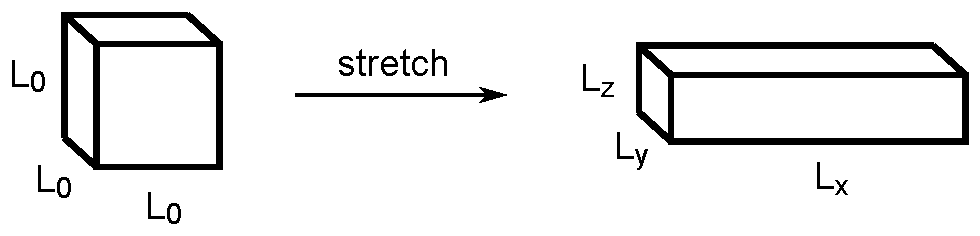
\includegraphics[width=0.7\textwidth]{\figpath/Model1_extension.pdf}}
	
	Usually, because we would like to look at properties that don't depend on the exact dimensions of the sample we are studying, we work in terms of the \emph{ratios} of the final dimensions of the sample to the initial dimensions.
	
	For the sample shown above, the extension ratios are:
	\begin{align*}
		\lambda_x = \frac{L_x}{L_0} && \lambda_y = \frac{L_y}{L_0} && \lambda_z = \frac{L_z}{L_0}
	\end{align*}
	These relationships allow us to write the final dimensions of the sample as
	\begin{align*}
		L_x = \lambda_x L_0 && L_y = \lambda_y L_0 && L_z = \lambda_z L_0
	\end{align*}
	
\end{model}


\begin{ctqs}

	\question First, consider the properties of the macroscopic sample.
	
		\begin{enumerate}
		
			\item What is the volume of the polymer sample depicted in Model \ref{\labelbase:mdl:macrostretch} before it is stretched?  Give your answer in terms of $L_0$.
	
		\begin{solution}[0.5in]
		
			$V = L_0^3$
		\end{solution}
	
			\item What is the volume of the polymer sample after it is stretched? Give your answer in terms of $L_x$, $L_y$, and $L_z$.
	
		\begin{solution}[0.5in]
		
			$V = L_x L_y L_z$
		\end{solution}
	
			\item There is usually no change in volume when we deform a bulk polymer network.  Write a mathematical relationship expressing this fact.
		\label{\labelbase:ctq:equalvolumes}
	
		\begin{solution}[0.5in]
			$L_0^3 = L_x L_y L_z$
		\end{solution}
		
			\item Use this information in Model \ref{\labelbase:mdl:macrostretch} to rewrite your the relationship from CTQ \ref{\labelbase:ctq:equalvolumes} in terms of $\lambda_x$, $\lambda_y$, and $\lambda_z$, and simplify as much as possible.
	
		\begin{solution}[1.5in]
			\begin{align*}
				L_0^3 &= (\lambda_x L_0)(\lambda_y L_0)(\lambda_z L_0) \\
				L_0^3 & = \lambda_x \lambda_y \lambda_z L_0^3 \\
				1 &= \lambda_x \lambda_y \lambda_z
			\end{align*}
		\end{solution}
		
		\end{enumerate}
	
	\question Next, consider the properties of a single polymer strand within the material.
	
		\begin{enumerate}
			
			\item If the polymer strand initially has end-to-end vector $\vec h_0 = (x_0, y_0, z_0)$, what do you expect its final end-to-end vector $\vec h$ will be, if the polymer strand stretches by the same ratios that the macroscopic sample does?  
			
			\emph{(Note: this assumption, that the individual chains stretch by the same ratios as the macroscopic sample, is referred to as \emph{affine deformation}.)}
		
			\begin{solution}[1in]
				$\vec h = (\lambda_x x_0, \lambda_y y_0, \lambda_z z_0)$
			\end{solution}
			
			\item Recall that when a single strand of polymer is stretched from end-to-end distance $h$ to end-to-end distance $h_0$, its change in entropy is 
			\begin{equation*}
				\Delta S_{strand} = -k\left(\frac{3}{2Nb^2}\right)(h^2 - h_0^2)
			\end{equation*}
			 What is $\Delta S_{strand}$ in terms of $x_0$, $y_0$, $z_0$ and $\lambda_x$, $\lambda_y$, and $\lambda_z$?  Write out all of the terms, but do not worry about simplifying your answer.
		
				\begin{solution}[2.25in]
					\begin{align*}
						\Delta S_{strand} &= -k\left(\frac{3}{2Nb^2}\right)(h^2 - h_0^2)\\
							&= -k\left(\frac{3}{2Nb^2}\right)\left(\left(((\lambda_x x_0)^2 + (\lambda_y y_0)^2 + (\lambda_z z_0)^2\right) - \left(x_0^2 + y_0^2 + z_0^2\right)\right)
					\end{align*}
				\end{solution}
				
		\end{enumerate}
				
\end{ctqs}

\begin{infobox}

	For the rest of this activity, we will consider \emph{uniaxial} extension, in which $\lambda_x \equiv \lambda$ and $\lambda_y = \lambda_z = \frac{1}{\sqrt{\lambda}}$ (these latter two relationships are necessary to ensure that the volume of the sample does not change, as you explored in CTQ \ref{\labelbase:ctq:equalvolumes}).  In this case, it is possible to show that
	
		\begin{equation*}	
				\Delta S_{strand} = -\frac{k}{2}\left(\lambda^2 + \frac{2}{\lambda} - 3\right)
			\label{\labelbase:eqn:delSstranduniaxial}
		\end{equation*}
			
\end{infobox}

\begin{ctqs}
		
	\question Suppose that there are a total of $v_e$ polymer strands that stretch when the material is stretched (we refer to these as ``elastically-effective'' strands). What will the total entropy change of the network ($\Delta S_{network}$) be, in terms of $v_e$, $\lambda$, and any other necessary constants?
		
			\begin{solution}[1.5in]
				\begin{align*}
					\Delta S_{network} &= v_e \Delta S_{strand}\\
						&= -\frac{v_e k}{2}\left(\lambda^2 + \frac{2}{\lambda} - 3\right)
				\end{align*}
			\end{solution}
		
	\question Finally, recalling that $f = -T\left(\frac{\partial S}{\partial L}\right)$, find an expression for the force required to stretch the material by extension ratio $\lambda$.
	
		\emph{Hint: Because $L = \lambda L_0$, we can also write $f$ as $f = -\frac{T}{L_0}\frac{\partial \Delta S}{\partial \lambda}$, which will be the easier form to use for this problem.}
		
			\begin{solution}[3in]
			
				\begin{align*}
					f &= -\frac{T}{L_0}\frac{\partial}{\partial \lambda} \left(-\frac{v_e k}{2}\left(\lambda^2 + \frac{2}{\lambda} - 3\right)\right)\\
						&= \frac{T}{L_0}\frac{v_e k}{2}\frac{\partial}{\partial \lambda} \left(\left(\lambda^2 + \frac{2}{\lambda} - 3\right)\right)\\
						&= \frac{v_e k T}{2 L_0}\left(2\lambda - \frac{2}{\lambda^2} \right)\\
						&= \frac{v_e k T}{L_0}\left(\lambda - \frac{1}{\lambda^2} \right)
				\end{align*}
			\end{solution}
	
\end{ctqs}

\begin{model}[Stress and Strain]

	In most experiments, we usually report our data in terms of the \emph{stress} and \emph{strain} on the material, which normalize the force (stress) and change in length (strain) to the initial dimensions of the sample.
	
	The stress and strain are defined as follows:
	\begin{align*}
		\text{stress:} && \sigma = \frac{\text{force}}{\text{initial cross-sectional area}} = \frac{f}{L_0^2} \\
		\text{strain:} && \epsilon = \frac{\text{change in length}}{\text{initial length}} = \frac{L-L_0}{L_0}
	\end{align*}
	
\end{model}

\begin{ctqs}

	\question Write an expression for the stress, $\sigma$, in terms of $v_e$, $\lambda$, $L_0$, and any other necessary constants.
	
		\begin{solution}[0.8in]
			\begin{equation*}
				\sigma = kT\frac{v_e}{L_0^3}\left(\lambda - \frac{1}{\lambda^2}\right)
			\end{equation*}
		\end{solution}

	\question Write an expression for the strain, $\epsilon$, in terms of $\lambda$ and any other necessary constants.
	
		\begin{solution}[0.8in]
			\begin{equation*}
				\epsilon = \frac{L-L_0}{L_0} = \frac{L}{L_0} -1 = \lambda - 1
			\end{equation*}
		\end{solution}
		
	\question Recall that polymers behave like springs.  Hooke's law states that the relationship between force ($f$) and deformation ($x$) of a spring follows $f=kx$, where $k$ is an appropriate spring constant.
	
		Propose an equivalent relationship for stress and strain, using the \emph{Young's Modulus}, $E$, in place of the spring constant.
		
			\begin{solution}[0.5in]
			
				$\sigma = E\epsilon$
				
			\end{solution}
	
\end{ctqs}

\begin{infobox}
	For small deformations ($\lambda$ close to 1), it is possible to show that
	\begin{equation*}
		E \approx 3kT\frac{v_e}{V}
	\end{equation*}
	where $v_e$ is the total number of elastically-effective strands, and $V$ is the volume of the sample.
\end{infobox}

\begin{ctqs}
	\question Will the material become easier or harder to stretch as temperature is increased?  Explain your group's reasoning in 1-2 complete sentences.
	
		\begin{solution}[1.5in]
			The solution will become more difficult to stretch as temperature is increased.  Increasing $T$ increases the Young's modulus, which effectively makes the polymer behave as a stiffer spring.
		\end{solution}
	
	\question In 2-3 complete sentences, propose an experiment that you could do to measure the number of elastically-effective chains per unit volume in an unknown polymer sample.
	
		\begin{solution}[1.75in]
		
			To measure the number of elastically-effective chains per unit volume, we could slowly stretch the material while measuring the required force.  We could then convert the measured force at each extension to a stress (and strain), and fit the data to a line.  The slope of this line would give us the Young's modulus, and we could then divide by $3kT$ to get the number of elastically-effective chains per unit volume.
		
		\end{solution}
\end{ctqs}


\begin{exercises}

	\exercise Experimentally, we find that the number of \emph{elastically-effective} strands in a polymer network is always smaller than the \emph{total} number of strands in the network.  Using your knowledge of the structural features of polymer networks, suggest at least one reason that this might be true.
	
		\begin{solution}
			\instructordisplay{Some strands in the polymer network may form loops, which will not stretch when the material is stretched.  These strands will not be elastically effective, making the number of elastically-effective strands smaller than the total number of strands in the network.
			
			Note: alternatively, students may answer in terms of dangling ends, or sol fraction; both of these are also appropriate answers to this question.}
		\end{solution}
	
	%\exercise Derive expression for $\Delta S_{strand}$ for uniaxial extension
	
	%\exercise Derive expression for $E$ at low strain
	
	%\exercise analyze experimental tensile data to extract Young's modulus
	
	\exercise Often, it is more useful to think about polymer networks in terms of the average \emph{molecular weight between crosslinks} rather than the number of elastically effective strands per unit volume.
	
		\begin{enumerate}
			\item Suppose your polymer of interest has density $\rho$.  What is the total mass of a sample of volume $V$?
			
				\begin{solution}
					\instructordisplay{$\rho V$}
				\end{solution}
			
			\item How many chains of molecular weight $M_x$ would be contained in a sample of volume $V$?  Give your answer in terms of the  number of individual chains, not just moles of chains.
			
				\begin{solution}
					\instructordisplay{$\frac{N_{av} \rho V}{M_x}$
					
					(note: $N_{av}$ is Avogadro's number)}
				\end{solution}
			
			\item Assuming all of these chains are elastically effective (i.e. that the number you calculated in the previous part is equal to $v_e$), find an expression for the number of elastically effective chains per unit volume in terms of the polymer density, the molecular weight between crosslinks, and any other necessary constants.
			
				\begin{solution}
					\instructordisplay{$\frac{v_e}{V} = \frac{1}{V}\left(\frac{N_{av} \rho V}{M_x}\right) = \frac{N_{av} \rho}{M_x}$}
				\end{solution}
		\end{enumerate}
	
\end{exercises}


%\begin{problems}
%
%	\problem First exercise
%	\problem Second exercise
%	
%\end{problems}


	
\end{activity}


\end{document}
